\documentclass[a4paper, 12pt]{article}
\usepackage{fancyhdr}
\usepackage[MeX]{polski}
\usepackage[utf8]{inputenc}
\usepackage{amsmath,amsthm,amssymb}
\usepackage{graphicx}
\usepackage{multirow}
\usepackage[lmargin=2.7cm]{geometry}
\usepackage{color}

\pagestyle{fancy}
\lhead{\textbf{Wtomigraj} -- Opis architektury}
\rhead{\bfseries}

\author{Marcin Januszkiewicz, Grzegorz Łoś}
\title{\textbf{Wtomigraj} -- Opis architektury}

\newcommand{\newtitle}[1]{
\begin{center}
\thispagestyle{empty}
{\Large Licencjacka Pracownia Oprogramowania, zespół 21}\\[0.5cm]
{\Large Instytut Informatyki Uniwersytetu Wrocławskiego 2011/12}\\[2.5cm]
{\huge Dokumentacja projektu \textbf{Wtomigraj}}\\[0.5cm]
{\huge #1}\\[0.5cm]
{\large Marcin Januszkiewicz, Grzegorz Łoś}\\[0.5cm]
\vfill
{\large Wrocław, \today}
\end{center}
\newpage
}
\renewcommand{\thesection}{\arabic{section}.}
\renewcommand{\thesubsection}{\arabic{section}.\arabic{subsection}.}
\renewcommand{\thesubsubsection}{\arabic{section}.\arabic{subsection}.\arabic{subsubsection}.}


\begin{document}

%\makeatletter
 %   \renewcommand\@seccntformat[1]{\csname the#1\endcsname.\quad}
  %  \renewcommand\numberline[1]{#1.\hskip0.7em}
%\makeatother

\newtitle{Architektura projektu}

\setcounter{page}{2}

\tableofcontents

\break

\section{Ogólny opis architektury}

Każdy klient może zostać gospodarzem nowej gry lub przyłączyć się do nierozpoczętej gry (mówimy wtedy, że jest gościem). Kiedy do nierozpoczętej partii dołączy minimalna liczba wymaganych graczy (zależy ona od gry), to partia może zostać rozpoczęta. Serwer służy tylko jako pośrednik w nawiązaniu połączenia pomiędzy graczami zainteresowanymi odbyciem wspólnej partii, nie ma żadnego udziału w jej przebiegu. Wszyscy goście komunikują się wyłącznie z gospodarzem. Wszystkie obiekty związane z grą znajdują się w pamięci komputera gospodarza. Klient gospodarza wysyła gościom informacje o zmianach stanów tych obiektów, a klienci-goście wyświetlają je swoim użytkownikom na ekranach monitorów i przekazują gospodarzowi ich ruchy. Po zakończeniu gry wszyscy klienci ponownie komunikują się z serwerem, który może pośredniczyć w zainicjowaniu kolejnej partii. Schemat architektury przedestawiono na rysunku~\ref{fig:arch}.

Końcowymi użytkownikami są internauci pragnący pograć z innymi. Programista gry korzystający z platformy Wtomigraj powinien na wydzielonym serwerze uruchomić program serwera oraz udostępnić użytkownikom grę, na przykład w postaci aplikacji okienkowej w pakiecie jar lub jako aplet osadzony na stronie internetowej.

\begin{figure}
\centering
\caption{Schemat komunikacji klientów i serwera}
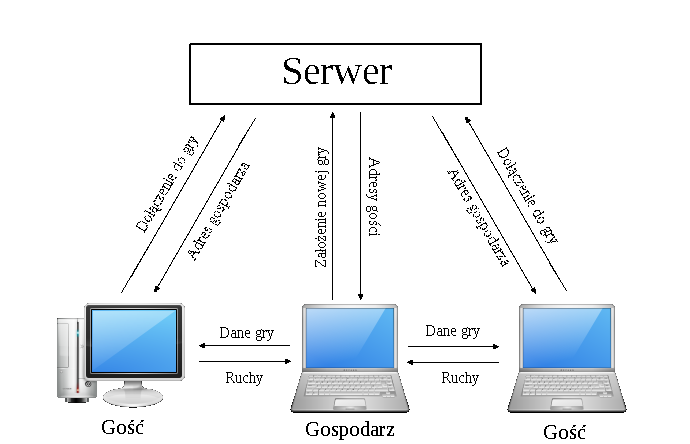
\includegraphics[scale=0.6]{rysunki/arch.png}
\label{fig:arch}
\end{figure}

\subsection{Stany partii}
Partia może znajdować się w jednym z trzech stanów:
\begin{enumerate}
 \item \textbf{Nierozpoczęta.} W tym stanie do rozgrywki mogą dołączać gracze. Nazwa rozgrywki jest widoczna w aplikacjach klientów znajdujących się w trybie menu. Gospodarz rozgrywki może ustawiać parametry związane z grą. 

 \item \textbf{Rozpoczęta.} Nazwa rozgrywki znika z listy widocznej na rysunku~\ref{fig:menu}, użytkownicy tracą możliwość dołącznia do niej. Gospodarz otrzymuje od serwera adresy gości, a goście adres gospodarza. Na komputerze gospodarza inicjowane są wszystkie obiekty związane z grą i partia się rozpoczyna.

 \item \textbf{Zakończona.} Rozgrywka się zakończyła, lecz gospodarz jeszcze jej nie opuścił. W tym stanie gracze mogą oglądać wyniki, analizować statystyki gry lub dyskutować nad przebiegiem partii.
\end{enumerate}

\subsection{Tryby klienta}
Aplikacja klienta w każdym momencie znajduje się w jednym z trzech trybów.

\paragraph{Tryb menu.} Jest to tryb pomiędzy partiami.

Aplikacja prezentuje swojemu użytkownikowi rozgrywki, do których może się przyłączyć, daje możliwość rozpoczęcia nowej rozgrywki oraz porozmawiania z pozostałymi graczami. Przedstawiono to na rysunku~\ref{fig:menu}. 

\paragraph{Tryb gospodarza.} W tym trybie klient staje się gospodarzem partii. Początkowo oczekuje aż dołączy odpowiednio wielu graczy. Użytkownicy, których klienci znajdują się w trybie menu, widzą tę partię na swoim panelu i mogą do niej dołączyć. W tym czasie gospodarz może ustawić parametry związane z grą, co przedstawia rysunek~\ref{fig:inicjacja}.


Po pojawieniu się wymaganej liczby graczy partia może zostać rozpoczęta. Znika wówczas z listy dostępnych gier. Aplikacja gospodarza odpowiada za wykonywanie wszelkich obliczeń i operacji związanych z grą. Wszystkich gości informuje tylko o~zmianach stanów istotnych obiektów, tak aby aplikacje gości mogły je należycie wyświetlić swoim użytkownikom. Goście przekazują swoje ruchy gospodarzowi, który uwzględnia je w logice gry. Ponadto aplikacja w trybie hosta wykonuje te same zadania, co aplikacja w trybie gościa, ponieważ jej użytkownik także jest graczem.

\paragraph{Tryb gościa.} W tym trybie aplikacja służy do wyświetlania stanu gry swojemu użytkownikowi oraz przekazywania jego ruchów gospodarzowi partii.


\begin{figure}
\centering
\caption{Aplikacja w stanie menu}
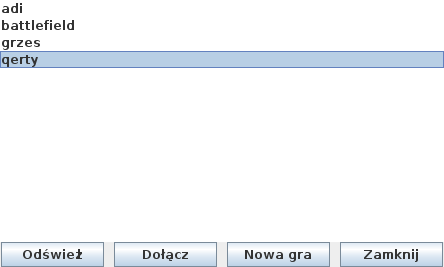
\includegraphics[scale=0.8]{rysunki/menu.png}
\label{fig:menu}
\end{figure}


\begin{figure}
\centering
\caption{Przykładowy panel gospodarza przed rozpoczęciem rozgrywki}
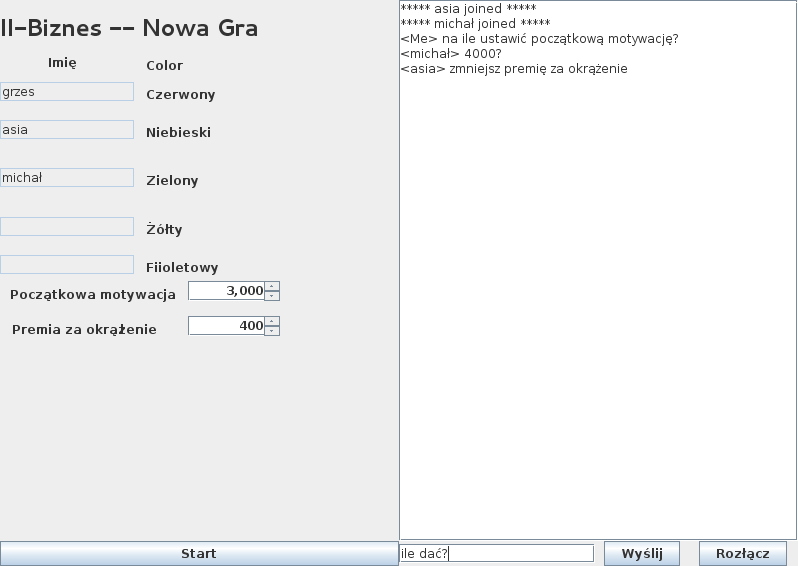
\includegraphics[scale=0.8]{rysunki/inicjacja.png}
\label{fig:inicjacja}
\end{figure}
\vspace{2cm}
\section{Zadania elementów systemu}

\paragraph{Serwer.} Służy skomunikowaniu aplikacji klientów. Może obsługiwać dowolnie wiele rodzajów gier.
Serwer:

\begin{itemize}
 \item przechowuje adresy klientów, ich pseudonimy, oraz odnośniki do partii w jakich się znajdują,
 \item rozsyła listę dostępnych partii pożądanej gry (aplikacja klienta wysyła informację do serwera jaka gra ją interesuje, bo serwer może jednocześnie służyć np. szachistom i brydżystom),
 \item pośredniczy w nawiązaniu komunikacji przez gospodarza i gościa.
\end{itemize}

\paragraph{Aplikacja klienta.} Jest implementacją pewnej gry, korzystającą ze stworzonej przez nas biblioteki do komunikacji. 

\begin{enumerate}
 \item W trybie menu:
    \begin{itemize}
      \item umożliwia tekstową komunikację użytkowników w okienku czata,
      \item przedstawia listę nierozpoczętych partii,
      \item daje możliwość dołączenia do nierozpoczętej partii lub założenia nowej.
    \end{itemize}

 \item W trybie gospodarza:
    \begin{itemize}
      \item przechowuje adresy klientów gości,
      \item trzyma w pamięci wszystkie obiekty związane z partią, 
      \item służy ustawieniu parametrów partii i jej rozpoczęciu,
      \item odpowiada za uaktualnianie logiki rozgrywki,
      \item przyjmuje od gości informacje o ich ruchach,
      \item wysyła gościom informacje o aktualnym stanie partii,
      \item pełni także funkcje klienta w trybie gościa, ponieważ gospodarz także jest graczem.
    \end{itemize}

 \item W trybie gościa:
    \begin{itemize}
      \item przechowuje adres gospodarza,
      \item przyjmuje od gospodarza komunikaty o aktualnym stanie partii,
      \item wyświetla użytkownikowi stan gry (na przykład w przypadku szachów będzie do rysunek szachownicy i bierek),
      \item oczekuje na ruchy swojego użytkownika (w przypadku szachów kliknięcia na bierki i pola), a następnie wysyła je gospodarzowi.
    \end{itemize}
\end{enumerate}


\section{Opis protokołu}
Komunikacja pomiędzy klientem a serwerem odywa się przez wymianę pakietów UDP z wiadomościami zawartymi w polach danych. W warstwie aplikacji protokół ma formę pytanie-odpowiedź, co zapewnia odporność na błędy sieci związane ze stratą pakietów. Wiadomości przesyłane są w formacie JSON, co pozwala na wykorzystanie istniejących bibliotek do prostego kodowania i dekodowania informacji.

Każdy obiekt JSON zawiera pola:
\begin{itemize}
 \item \texttt{type} -- typ komunikatu, łańcuch znaków. Wszystkie typy komunikatów omawiamy poniżej,
 \item \texttt{res} -- pole boolowskie ustawione na true, gdy pakiet jest odpowiedzią, w przeciwnym razie jest to pytanie,
 \item \texttt{id} -- w przypadku pakietów-pytań jest to numer identyfikacyjny pytania, natomiast dla odpowiedzi oznacza identyfikator pytania, na które odpowiadamy.
\end{itemize}
Ponadto dla każdego typu komunikatu obiekt JSON może zawierać dodatkowe pola.

\paragraph{Inne pola.} Opisane poniżej pola występują w niektórych typach komunikatów.
\begin{itemize}
 \item \texttt{nick} -- pseudonim używany przez klienta.
 \item \texttt{name} -- nazwa partii, do której odnosi się komunikat.
 \item \texttt{game} -- nazwa (rodzaj) gry, do której odnosi się komunikat.
 \item \texttt{channels} -- lista nazw partii, do których może dołączyć klient. 
 \item \texttt{desc} -- słowny opis komunikatu.
\end{itemize}

\subsection{Typy komunikatów}
\paragraph{Komunikaty wysyłane przez klienta do serwera.}
\begin{description}
 \item[newclient] -- komunikat informujący o chęci przyłączenia się do serwera. Zawiera pole \texttt{nick} (pożądany pseudonim).
 \item[newchannel] -- komunikat będący prośbą o założenie nowej partii. Zawiera pola \texttt{name} oraz \texttt{game}.
 \item[join] -- komunikat będący prośbą o przyłączenie do partii. Zawiera pola \texttt{name} oraz \texttt{game}.
 \item[exit] -- komunikat będący informacją o odłączeniu od partii.
 \item[sendchannels] -- komunikat będący prośbą o przesłanie listy partii do których może dołączyć klient. Zawiera pole \texttt{game}.
 \item[emptyresponse] -- komunikat wysyłany w odpowiedzi na pytania, które \textit{de facto} są polecaniami i nie wymagają żadnej odpowiedzi, prócz potwierdzenia, że pakiet doszedł, np. \textbf{echorequest}, \textbf{channelcanceled}.
\end{description}


\paragraph{Komunikaty wysyłane przez serwera do klienta.}
\begin{description}
 \item[welcome] -- odpowiedź na \textbf{newclient}. Komunikat ten oznacza, że serwer zaakceptował wybrany identyfikator. Dla potwierdzenia znajduje się on w polu \texttt{nick}. Ponadto pakiet zawiera pole \texttt{channels}.
 \item[invalidnick] -- odpowiedź na \textbf{newclient}. Komunikat ten oznacza, że wybrany identyfikator nie został zaakceptowany. Zawiera pola \texttt{errid} oraz \texttt{desc} oznaczające numer błędu oraz jego opis.
 \item[echorequest] -- komunikat żądający od klienta potwierdzenia swojej obecności.
 \item[channellist] -- odpowiedź na \textbf{sendchannels}. Zawiera pole \texttt{channels}.
 \item[channelaccepted] -- odpowiedź na \textbf{newchannel}. Komunikat ten oznacza, że serwer akceptuje założenie przez klienta nowego kanału rozmowy.
  \item[channelrejected] -- odpowiedź na \textbf{newchannel}. Komunikat ten oznacza, że serwer odrzuca założenie przez klienta nowego kanału rozmowy. W treści komunikatu przesyłany jest numer błędu i jego opis.
 \item[joinaccepted] -- odpowiedź na \textbf{join}. Komunikat ten oznacza, że prośba klienta o dołączenie do pewnego kanału została zaakceptowana. W polu \texttt{name}, jako potwierdzenie, znajduje się nazwa kanału, do którego dołącza klient.
  \item[joinrejected] -- odpowiedź na \textbf{join}. Komunikat ten oznacza, że prośba klienta o dołączenie do pewnego kanału została odrzucona.Zawiera pola \texttt{errid} oraz \texttt{desc} oznaczające numer błędu oraz jego opis.
 \item[exitaccepted] -- odpowiedź na \textbf{exit}. Oznacza on, że klient został wypisany z kanału rozmowy. Ponadto w polu \texttt{channels} zawarta jest lista nazw kanałów, do których może dołączyć klient.
 \item[address] -- Pakiet zawiera pola \texttt{address} oraz \texttt{port} będące adresem pewnego klienta. 
 \item[channelcanceled] -- komunikat informujący klienta, że partia w której się znajduje przestał istnieć.
 \item[userleft] -- komunikat informujący gospodarza, że partię w którym się znajduje opuścił użytkownik. W treści komunikatu przesyłany jest identyfikator odchodzącego użytkownika.
 \item[error] -- komunikat wysyłany gdy wystąpi bład inny niż te opisane wyżej. Zawiera pola \texttt{errid} oraz \texttt{desc} oznaczające numer błędu oraz jego opis.
\end{description}

\paragraph{Komunikaty wysyłane prez klienta do klienta.}
\begin{description}
 \item[holepunch] -- Pakiet, który ma na celu ,,wybicie dziury'' (opisane w dziale \ref{sec:komunikacja}).
 \item[icanhearyou] -- Odpowiedź na \textbf{holepunch}.
 \item[gamedata] -- pakiet zawierający dane gry. Pozostałe pola pakietu są zdefiniowane przez programistę gry.
\end{description}
 

\section{Komunikacja między serwerem i klientami}
\label{sec:komunikacja}

\subsection{Komunikaty z serwera do klienta}
Tabela~\ref{tab:serdokli} zawiera słowny opis komunikatów wysyłanych z serwera do klienta i pożądane zachowanie aplikacji klienta. 
\begin{table}
\begin{center}
 \begin{tabular}{p{2cm}||p{5.2cm}||p{7cm}}
 \hbox{Tryb} klienta& Rodzaj komunikatu & Co powinien zrobić klient\\ \hline \hline
\multirow{6}{*}{Menu}
  & Wiadomość
  & Wyświetlić ją w stosownym okienku \\ \cline{2-3}

  & Lista dostępnych rozgrywek
  & Wypisać je na przeznaczonej do tego liście \\ \cline{2-3}

  & Akceptacja utworzenia nowej rozgrywki
  & Przełączyć się w tryb gospodarza, wyświetlić panel z ustawieniami partii. \\ \cline{2-3}

  & Odrzucenie nowej partii
  & Wyświetlić komunikat z przyczyną \\ \cline{2-3}

  & Akceptacja dołączenia do rozgrywki 
  & Przejście w tryb gościa \\ \cline{2-3}

  & Odrzucenie prośby o dołącznie do rozgrywki
  & Wyświetlić komunikat z przyczyną \\ \hline \hline

\multirow{2}{*}{Gospodarz}
  & Dołączenie gracza
  & Sprawdzić czy można rozpocząć rozgrywkę \\ \cline{2-3}

  & Odejście gracza
  & Jeżeli partia nie jest rozpoczęta, to być może należy wyłączyć możliwość rozpoczęcia gry. Jeżeli jest rozpoczęta, to postępowanie zależy od konkretnej gry \\ \hline \hline

  Gość
  & Odejście gospodarza
  & Wyświetlić komunikat o przerwaniu gry i wrócić do trybu menu \\ \hline \hline
\end{tabular}
\caption{Komunikaty z serwera do klienta.}
\label{tab:serdokli}
\end{center}
\end{table}

\subsection{Komunikaty od klienta do serwera}
Tabela~\ref{tab:klidoser} zawiera słowny opis komunikatów wysyłanych od klienta do serwera i zachowanie serwera.

\begin{table}
\begin{center}
 \begin{tabular}{p{2cm}||p{3.5cm}||p{9cm}}
 \hbox{Tryb} klienta& Rodzaj komunikatu & Co powinien zrobić serwer\\ \hline \hline
\multirow{3}{*}{Menu}
  & Rozpoczęcie nowej rozgrywki
  & Jeżeli nazwa gry jest poprawna, to:
      \begin{itemize}
      \item poinformować klienta o akceptacji rozgrywki,
      \item przesłać pozostałym klientom komunikat o nowej rozgrywce,
      \item utworzyć obiekt rozgrywki,
      \item przepisać klienta z listy wolnych do zajętych z referencją do utworzonej rozgrywki.
      \end{itemize}
    W przeciwnym razie wysłać klientowi komunikat o odrzuceniu rozgrywki \\ \cline{2-3}

  & Prośba o dołączenie do partii
  & Jeżeli z jakiegoś powodu klient nie może do niej dołączyć, to wysyłamy stosowny komunikat. W przeciwnym razie tworzymy odnośnik do partii, w której znajduje się klient\\ \hline

\multirow{2}{*}{Gospodarz}
  & Odejście z rozgrywki
  & Wszystkim gościom wysyłamy komunikat o odejściu gospodarza. Przepisujemy wszystkich z listy zajętych do wolnych i usuwamy obiekt rozgrywki.\\ \cline{2-3}

  & Rozpoczęcie rozgrywki
  & Informujemy wolnych klientów, że rozgrywka jest już nieaktualna.\\ \hline \hline

Gość & odejście z rozgrywki & Usuwamy klienta z list zajętych i umieszczamy na liście wolnych. Wysyłamy gospodarzowi rozgrywki komunikat o odejściu gościa.

\end{tabular}
\caption{Komunikaty od klienta do serwera.}
\label{tab:klidoser}
\end{center}
\end{table}


\subsection{Komunikacja gość-gospodarz}

\paragraph{Nawiązywanie połączenia między klientami.} W celu skomunikowania dwóch klientów korzystamy z metody ,,wybijania dziur'' (ang. \textit{holepunching}). Polega ona na tym, by do komputera, z którym chcemy się skontaktować wysyłać jakiekolwiek pakiety (ich zawartość jest nieważna). Robimy tak ze względu na to, że rutery często odrzucają pakiety od nieznanego nadawcy. Jednak kiedy ruter zobaczy, że otrzymujemy pakiet z adresu, do którego my także już coś wysyłaliśmy, to adres ten uzna za zaufany i pakiety zaczną przechodzić. 

Komunikacja między gospodarzem i jego gośćmi w trakcie partii może być dowolnie zdefiniowana przez programistę gry.

\subsection{Zerwanie połączenia}
W przypadku, gdy połączenie z klientem zostanie przerwane serwer musi podjąć pewne działania. Jeśli klient znajdował się w trybie:
\begin{itemize}
 \item \textbf{gospodarza} -- powiadamiamy wszystkich gości w partii o jego odejściu i usuwamy partię.
 \item \textbf{gościa} -- powiadamiamy gospodarza o odejściu klienta.
\end{itemize}
Serwer usuwa adres klienta z pamięci.


\section{Słownik}
\begin{description}
 \item[Gra] - rodzaj zabawy towarzyskiej, u nas internetowej, odbywający się według określonych reguł, na przykład: szachy, chińczyk.
 \item[Partia] - jest to przebieg pewnej gry, na przykład: partia szachów.
 \item[Gospodarz] - klient, na którego komputerze odbywa się logika rozgrywki.
 \item[Gość] - klient biorący udział w rozgrywce, niebędący gospodarzem.
 \item[Logika gry] - stan partii, wartości wszystkich obiektów związanych z partią.
\end{description}

\end{document} 
